\section{Aufbau und Durchführung}
\label{sec:Durchführung}
\subsection{Aufbau}
Um die Trägheitsmomente verschiedener Körper zu bestimmen, wird eine Drillachse wie in Abbildung \ref{df:1} verwendet.

\begin{figure}
  \centering
  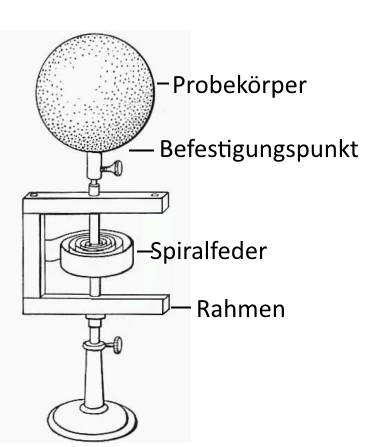
\includegraphics[height=7cm]{Aufbau.png}
  \caption{Drillachse.\cite{sample}}
  \label{df:1}
\end{figure}

Der zu untersuchende Körper wird auf eine drehbare Achse montiert, welche mit einer Spiralfeder am Rahmen befestigt ist.
Die Winkelrichtgröße $D$ und das Trägheitsmoment $I_{D}$ der Drillachse müssen jedoch noch bestimmt werden.
Es wird eine Winkelmessscheibe zwischen Körper und Rahmen angebracht, um die Auslenkungen des Körpers relativ zur Ruheposition bestimmen zu können.

\subsection{Durchführung}

\subsubsection{Bestimmung der Apperaturkonstanten}
Um die Winkelrichtgröße $D$ der Spiralfeder zu ermitteln, wird zunächst eine, hier angenommen masselose, Metallstange senkrecht zur Drehachse angebracht.
Senkrecht zu eben jener Metallstange wird in einem bestimmten Abstand zur Drehachse eine Federwaage mit einem Haken eingespannt.
Mit ihr wird die Drillachse um einen gewissen Winkel ausgelenkt.
Dies wird mit verschiedenen Abständen und Winkeln wiederholt, wobei jeweils die benötigte Kraft an der Federwaage abgelesen wird.\\
Das Eigenträgheitsmoment $I_{D}$ des Versuchsaufbaus wird dynamisch bestimmt.
Hierzu werden abgemessene Gewichte, welche als Punktmassen idealisiert werden, in jeweils gleichen bestimmten Abständen von der Drehachse angebracht.
Die Drillachse wird nun ausgelenkt und losgelassen.
Sie beginnt nun mit einer gewissen Periodendauer $T$ an zu schwingen.
Es wird die Zeit notiert, in der das System fünf volle Schwingungen durchläuft.
Dies wird ebenfalls für verschiedene Abstände der Massen zur Drehachse wiederholt.

\subsection{Bestimmung des Trägheitsmomentes zweier Körper}
Nun wird ein Körper oben an der Drehachse befestigt.
Wie zuvor wird eben jener relativ zur Ruheposition um einen Winkel ausgelenkt und es wird die fünffache Periodendauer $5T$ notiert.
Um das theoretische Trägheitsmoment des Körpers bestimmen zu können, müssen seine Maße bekannt sein.
Dazu wird seine Ausdehnung mittels Schieblehre und seine Masse mittels Waage bestimmt.
Dieses Experiment wird mit einem aufrechten Zylinder und einer Kugel durchgeführt.

\subsection{Bestimmung des Trägheitsmomentes einer Puppe}
Bei diesem Versuch steht als zu untersuchender Körper eine bewegliche Holzpuppe zur Verfügung.
Ihre Masse und ihre Maße werden wie zuvor bestimmt.
Die Puppe wird idealisiert durch Zylinder dargestellt.
Wie zuvor wird die fünffache Periodendauer ermittelt, jedoch wird dies für zwei Posen, welche in Abbildung \ref{df:2} dargestellt sind, wiederholt.

\begin{figure}
  \centering
  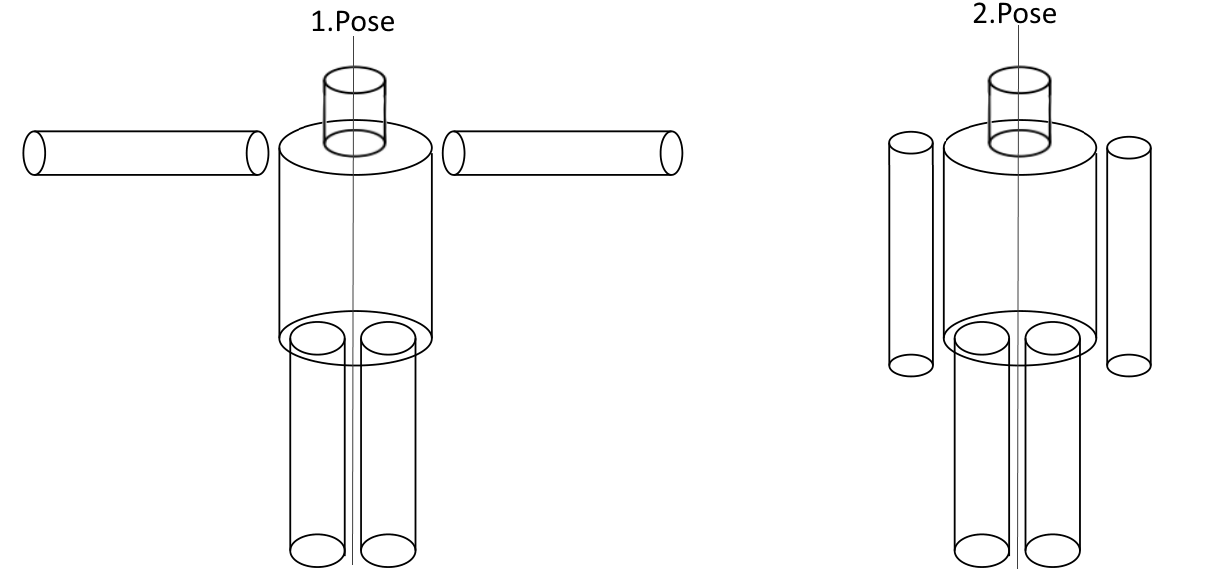
\includegraphics[height=7cm]{Posen.png}
  \caption{Posen der Holzpuppe.}
  \label{df:2}
\end{figure}
